\documentclass[a4paper,titlepage,twoside,12pt,leqno]{article}

\usepackage[]{fontspec}
\usepackage{xltxtra}
\usepackage[monogreek]{xgreek}

\newcommand{\en}[1]{\setlanguage{american}#1\setlanguage{monogreek}} % Για υφενώσεις στα αγγλικά

\defaultfontfeatures{Mapping=tex-text%, Scale=MatchLowercase}
} 

% Γραμματοσειρά
\setmainfont[Mapping=tex-text]{DejaVu Sans}


\usepackage{longtable} % για έναν μεγάλο πίνακα
\usepackage{graphicx, array, blindtext}

%Για την εντολή \caption* και την αφαίρεση του πίνακας 1:
\usepackage{caption}


\begin{document}

%Για την αφαίρεση της αρίθμησης των σελίδων
\pagestyle{empty}


\begin{table}[ht]
\caption*{\huge{Σύντομες οδηγίες εκκίνησης}}
\centering
\begin{tabular}{*{2}{m{0.48\textwidth}}}
\hline

\begin{center}\resizebox*{0.4\textwidth}{0.4\textwidth}{
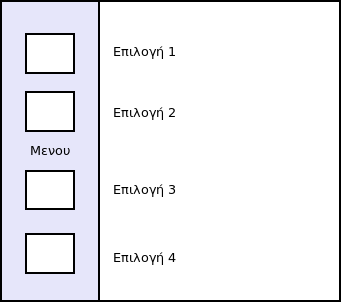
\includegraphics{images/menu.png}}\end{center} 

& \emph{Eισαγωγική οθόνη}

 Εδώ ο χρήστης μπορεί να περιηγηθεί στις κατηγορίες 
και να διαλέξει τί θέλει να κάνει \\
\hline

\begin{center}\rule{0.4\textwidth}{0.3\textwidth}\end{center} 

& \emph{Μενού παραγγελίας}

 Εδώ ο χρήστης μπορεί να περιηγηθεί στις κατηγορίες 
και να διαλέξει τί θέλει να κάνει \\
\hline

\begin{center}\rule{0.4\textwidth}{0.3\textwidth}\end{center} 

& \emph{Μενού παραγγελίας}

 Εδώ ο χρήστης μπορεί να περιηγηθεί στις κατηγορίες 
και να διαλέξει τί θέλει να κάνει \\
\hline

\begin{center}\rule{0.4\textwidth}{0.3\textwidth}\end{center} 

& \emph{Μενού παραγγελίας}

 Εδώ ο χρήστης μπορεί να περιηγηθεί στις κατηγορίες 
και να διαλέξει τί θέλει να κάνει \\
\hline

\end{tabular}
\label{table:getting_started}
\end{table}


\begin{table}[ht]
\centering
\begin{tabular}{*{2}{m{0.48\textwidth}}}
\hline

\begin{center}\rule{0.4\textwidth}{0.3\textwidth}\end{center} 

& \emph{Μενού παραγγελίας}

 Εδώ ο χρήστης μπορεί να περιηγηθεί στις κατηγορίες 
και να διαλέξει τί θέλει να κάνει \\
\hline


\end{tabular}
\label{table:getting_started}
\end{table}



\end{document}
